\index{GEF!Accessing Figures}
Although \gd{} supports identification and testing of GEF components out-of-the-box, it is highly recommend that application developers enhance this support by implementing an accessibility plug-in for their application. Such a plug-in makes identification of GEF components more robust and allows \gd{} tests to reference additional components, such as connection anchors. The following sections explain how to develop an accessibility plug-in.

\subsubsection{Setting up your Workspace}
% $Id: workspace.tex 1720 2006-03-02 12:25:33Z dennis $
% Local Variables:
% ispell-check-comments: nil
% Local IspellDict: american
% End:
% -----------------------------------------------------------
% copyright BREDEX GmbH 2004
% -----------------------------------------------------------
\item[Workspace]{Personal preferences relating to the client layout and 
actions are saved in a Workspace. All changes  made 
in the \bxcaption{Preferences}
dialog are stored here.
}


\subsubsection{Walkthrough}
The first step to implementing your accessibility plug-in is to create Identifiers for each type of GEF component that you wish to make accessible for \jb{} tests. An Identifier is a Java class that implements \bxname{com.bredexsw.guidancer.gef.identifier.IEditPartIdentifier} and provides \jb{} with additional and/or more precise information about a specific org.eclipse.gef.EditPart. The granularity of your Identifier classes will depend on the class hierarchy of the EditParts in the \gdaut{}. For example, if many of the EditParts share a common superclass, then you can write a single Identifier for that superclass that will be able to provide accessibility for all EditParts that inherit from that superclass. See \bxpref{gefreference} for a sample implementation.

The next step is to create an Adapter Factory. This extension will provide \jb{} with information regarding which Identifier to use for each Edit Part.
\begin{enumerate}
\item  Open the plugin.xml file for your accessibility plug-in and select the 'Extension' tab (\bxfigref{extensionstab}).

\begin{figure}[h]
\begin{center}
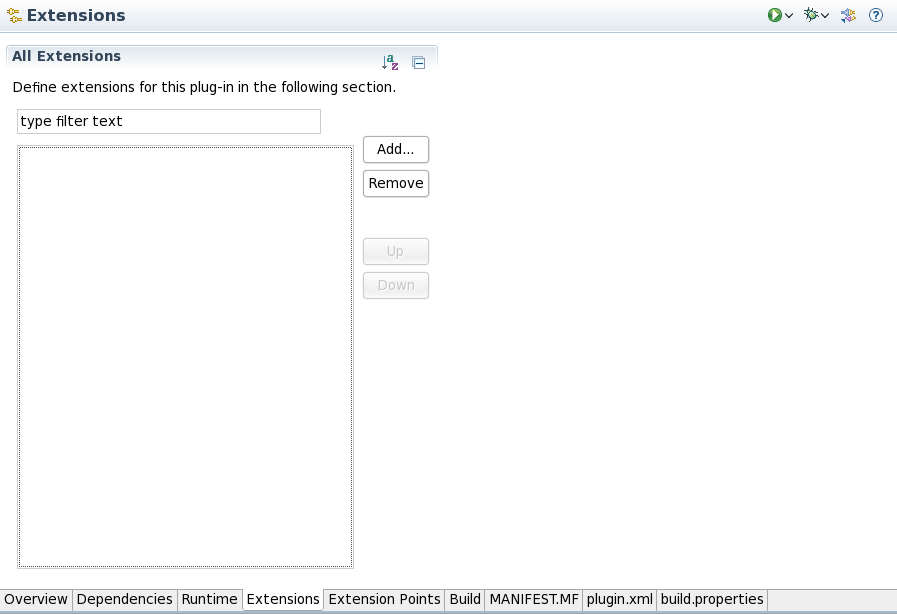
\includegraphics[width=12.5cm]{Tasks/GEF/PS/extensionstab}
\caption{Plug-in Editor with Extensions tab selected}
\label{extensionstab}
\end{center}
\end{figure}

\item Add an instance of the \bxname{org.eclipse.core.runtime.adapters} extension. 
\item Add a 'factory' to the new extension for each type of GEF component for which you wish to provide accessibility. Each factory must provide adapters from the GEF component that implements \bxname{org.eclipse.gef.EditPart} to \bxname{com.bredexsw.guidancer.gef.identifier.IEditPartIdentifier} (\bxfigref{factory}).

\begin{figure}[h]
\begin{center}
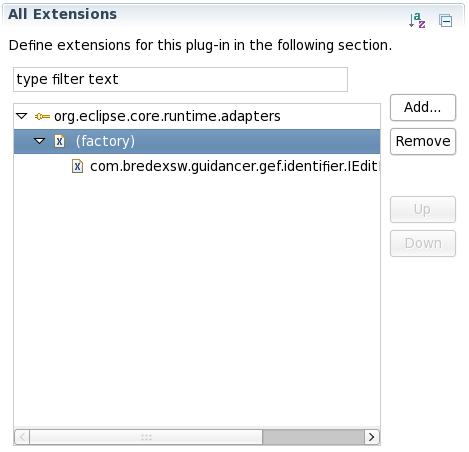
\includegraphics[width=12.5cm]{Tasks/GEF/PS/factory}
\caption{Plug-in Editor with defined Adapter Factory}
\label{factory}
\end{center}
\end{figure}

\item Once you have defined your Adapter Factory, you will need to implement it. Your Adapter Factory, which must implement \bxname{org.eclipse.core.runtime.IAdapaterFactory}, provides appropriate instances of your created Identifiers for a given Edit Part. See \bxpref{gefreference} for a sample implementation. 

\item Once you have created your Identifiers and Adapter Factories, you can export your plug-in and copy it to the 'plugins' directory of your \gdaut{} (\bxfigref{exportplugin}).

\bxtipp{When starting your \gdaut{} after adding or replacing your accessibility plug-in, it is recommended that the \gdaut{} be started with the -clean parameter.}

\begin{figure}[h]
\begin{center}
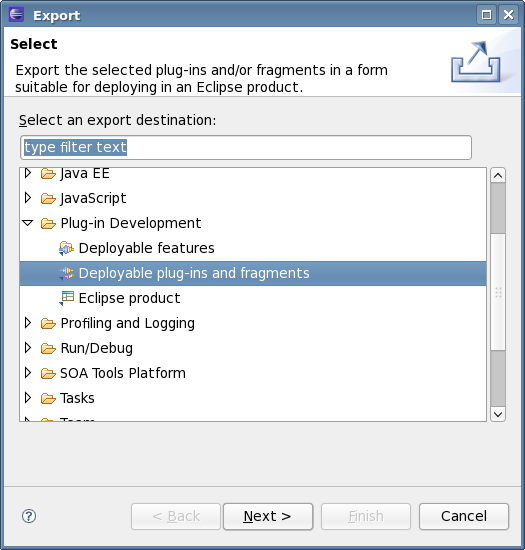
\includegraphics[width=12.5cm]{Tasks/GEF/PS/exportplugin}
\caption{Exporting the Project to a Plug-in}
\label{exportplugin}
\end{center}
\end{figure}

\end{enumerate}


\subsubsection{References}
\label{gefreference}
A sample accessibility plug-in for certain elements of the Logic Diagram sample plug-in project (contributed from the GEF plug-ins to Eclipse's New Project Wizard) are included in the installation. You can import the sample accessibility plug-in into an Eclipse workspace in order to examine the general structure of such an accessibility plug-in (\bxfigref{newlogicwizard})

\begin{figure}[h]
\begin{center}
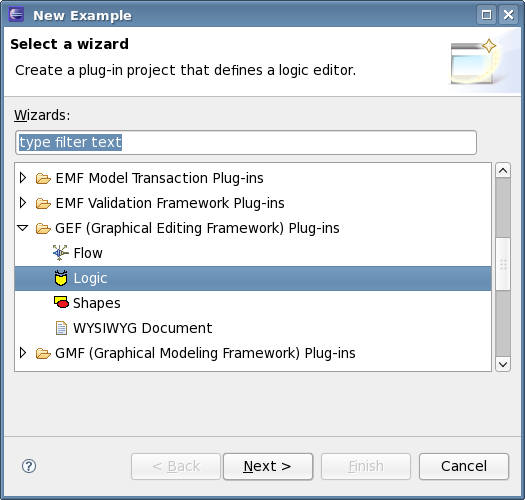
\includegraphics[width=12.5cm]{Toolkit/GEF/PS/newlogicwizard}
\caption{Creating the 'Logic' Project}
\label{newlogicwizard}
\end{center}
\end{figure}



The javadocs containing information about \bxname{org.eclipse.jubula.rc.rcp.gef.identifier.IEditPartIdentifier} and default implementations can be found in the installation directory under \bxname{documentation/gefapi/javadoc.zip}.
\clearpage

